\clearpage
\phantomsection
\label{202501121522}
\renewcommand{\notetitle}{Question-3}

\section*{Note Information}
\begin{itemize}
  \item \textbf{ID:} \texttt{202501121522}
  \item \textbf{Timestamp:} \texttt{\today \ \currenttime}
  \item \textbf{Tags:} \texttt{Tutoring, Chhean, Session-1}
  \item \textbf{References:}
    \begin{itemize}
      \item \href{}{}
    \end{itemize}
\end{itemize}


\section*{Main Content}
\textbf{Main Idea}\\
The velocity-time graph of a particle moving along a straight line is shown below. Time $t$ is measured in minutes, and the velocity $v(t)$ is measured in meters per minute.
\begin{center}
  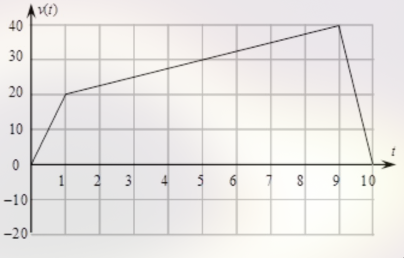
\includegraphics[width=0.5\textwidth]{Figures/Question-3.png}
\end{center}
If the average acceleration of the particle in the time interval $1 \leq t \leq 9$ minutes is $k$ m/min$^2$, the value of $k$ is 2.5 m/min$^2$.\\

\textbf{Explanation}\\
The average acceleartion can be calculated using the following formula:
\begin{align*}
  k = \frac{\Delta v}{\Delta t}\\ 
\end{align*}
According to the graph, $\Delta v = v(9) - v(1) = 40-20 = 20$. Thus,
\begin{align*}
  k = \frac{20}{8} = \frac{5}{2} = 2.5 \text{ m/min}^2
\end{align*}


\section*{Review}
\begin{enumerate}
  \item 
\end{enumerate}


\section*{Links to Other Notes}
\begin{itemize}
  \item \hyperref[]{}
\end{itemize}

\section*{Table of Contents}

\begin{itemize}
  \item \hyperref[toc]{TOC}
\end{itemize}

